%!TEX root = ../main.tex
\section{Introduction}
A common need when analysing real-world datasets is determining which instances stand out as being dissimilar to all others. Such instances are known as \emph{anomalies}, and the goal of \emph{anomaly detection} (also known as \emph{outlier detection}) is to determine all such instances in a data-driven fashion~\cite{chandola2007outlier}. Anomalies can be caused by errors in the data but sometimes are indicative of a new, previously unknown, underlying process; in fact Hawkins~\cite{hawkins} defines an outlier as an observation that {\it deviates so significantly from other observations as to arouse suspicion that it was generated by a different mechanism.} In the broader field of machine learning, the recent years have witnessed proliferation of deep neural networks, with unprecedented results across various application domains. Deep learning is subset of machine learning that achieves good performance and flexibility by learning to represent the data as nested hierarchy of concepts within layers of neural network. Deep learning outperforms the traditional machine learning as the scale of data increases as illustrated in Figure~\ref{fig:performanceCompare}. In recent years, deep learning-based anomaly detection algorithms has become increasingly popular and has been applied for diverse set of tasks as illustrated in Figure~\ref{fig:applications}; studies have shown that deep learning
completely surpasses traditional methods~\cite{javaid2016deep,peng2015multi}  in both research and applications ~\cite{javaid2016deep}.

% The answer to the question "Why is deep learning-based anomaly detection popular?" is mainly due to the following facets of deep learning-based approach:
% \begin{itemize}
% \item Deep learning-based anomaly detection algorithms learn hierarchical features from the data and such deep learned features potentially better capture complex relations hence improve the  discriminative abilities of the algorithms.
% \item Reduces feature engineering flaws, Consequently, some features that might not be apparent to a human view can be extracted easily by deep learning based models.
% \item Deep learning-based anomaly detection models improve the accuracy of the prediction model using large amount of data.
% \end{itemize}

% Compositional Structures of Social Dynamics are captured by deep learning methods and beat state-of-the-art methods~\cite{peng2015multi} , fails to capture the  temporal aspects of the
% data.

%performance comparision
\begin{figure}[h]
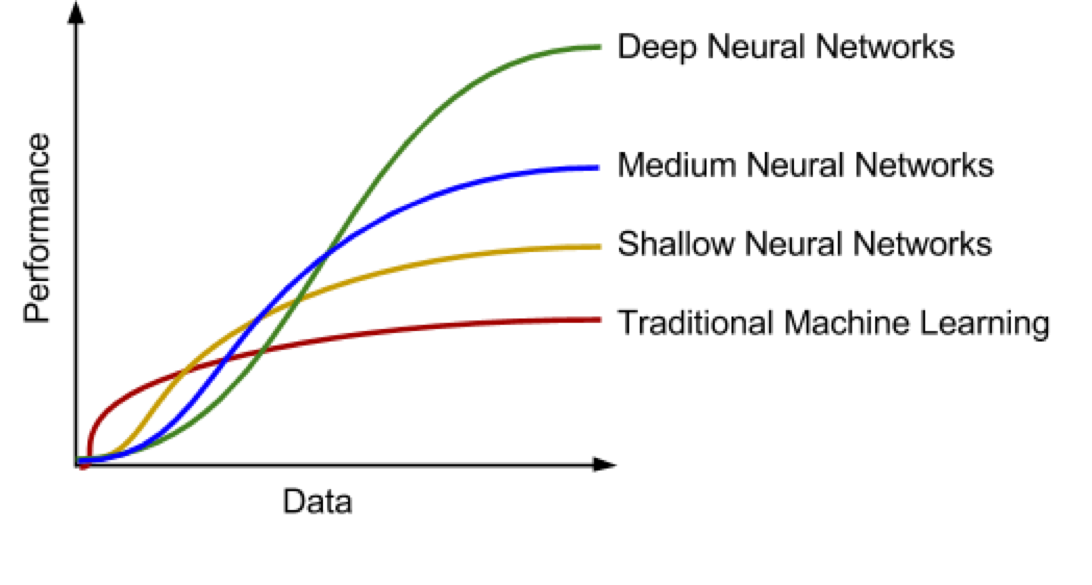
\includegraphics[scale=0.5]{images/traditionalVsDeepLearning}
\captionsetup{justification=centering}
\caption{Performance Comparision of Deep learning-based algorithms Vs Traditional Algorithms.}
\label{fig:performanceCompare}
\end{figure}


%%Applications of deep learning based anomaly detection
\begin{figure}[h]
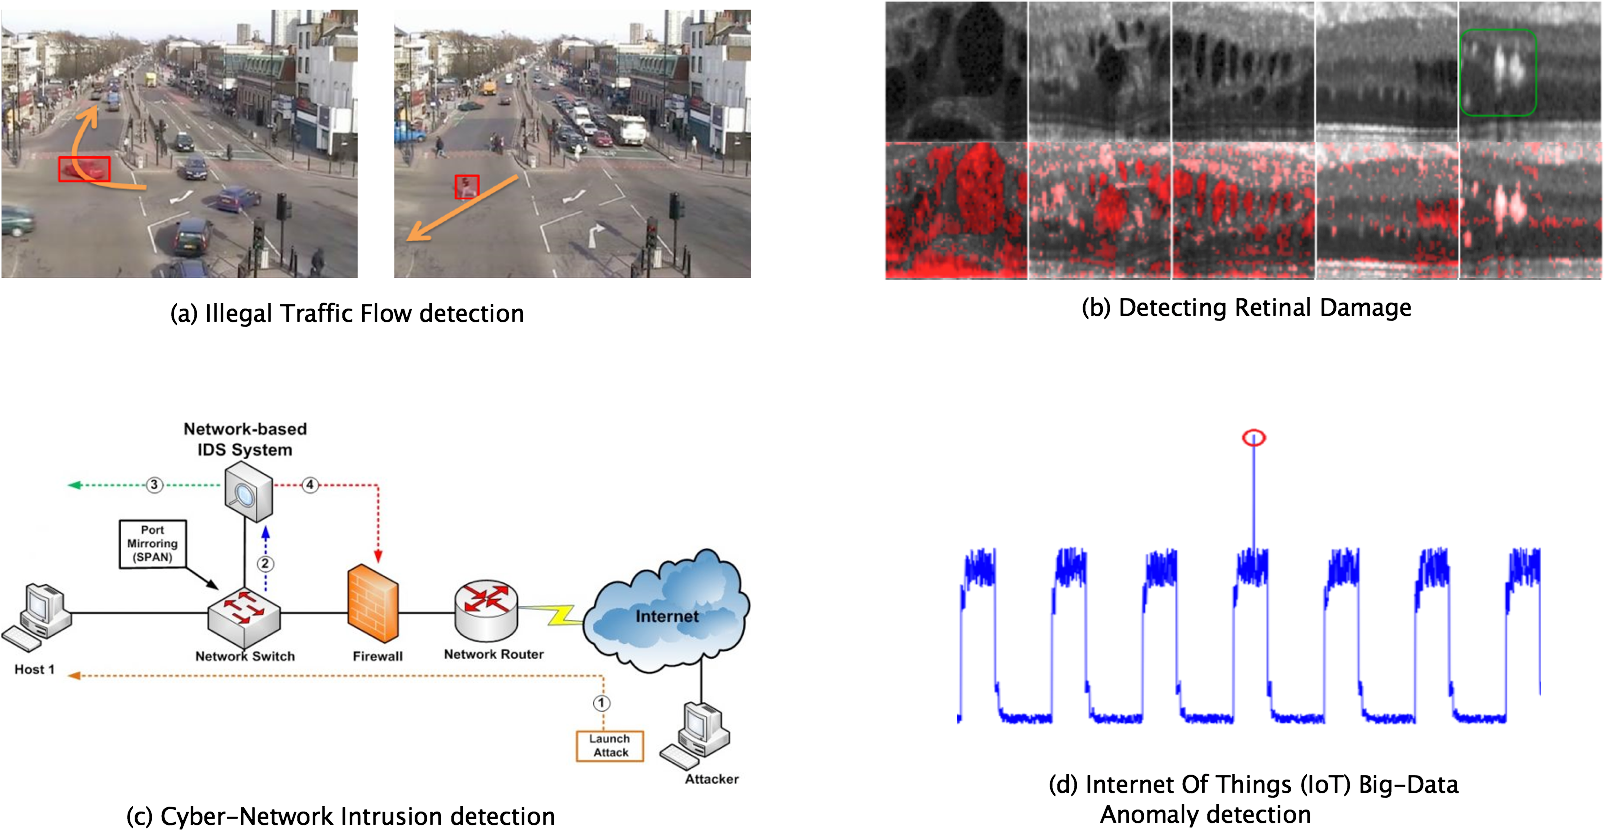
\includegraphics[scale=0.5]{images/applications}
\captionsetup{justification=centering}
\caption{Deep learning-based anomaly detection algorithms successfull applications.\\
(a) Video Survelliance, Image Analysis: Illegal Traffic detection~\cite{xie2017real}  ,  (b) Healthcare: Detecting Retinal Damage~\cite{schlegl2017unsupervised}\\
(c) Networks: Cyber-intrusion detection~\cite{javaid2016deep}  (d) Sensor Networks: Internet of Things (IoT) big-data anomaly detection~\cite{mohammadi2017deep} }
\label{fig:applications}
\end{figure}

The aim of this survey is two fold, firstly we present a structured and comprehensive overview of research methods in deep learning-based anomaly detection. Furthermore, we review the adoption of these deep-learning based methods for anomaly across various application domains and asess their effectiveness.

%anomalies
\subsection{ What are anomalies ?}
Anomalies  are also referred to as abnormalities, discordants, deviants, or outliers in the data mining and statistics literature~\cite{aggarwal2013introduction}.
% Anomaly Detection Definition
% \begin{figure}[h]
% 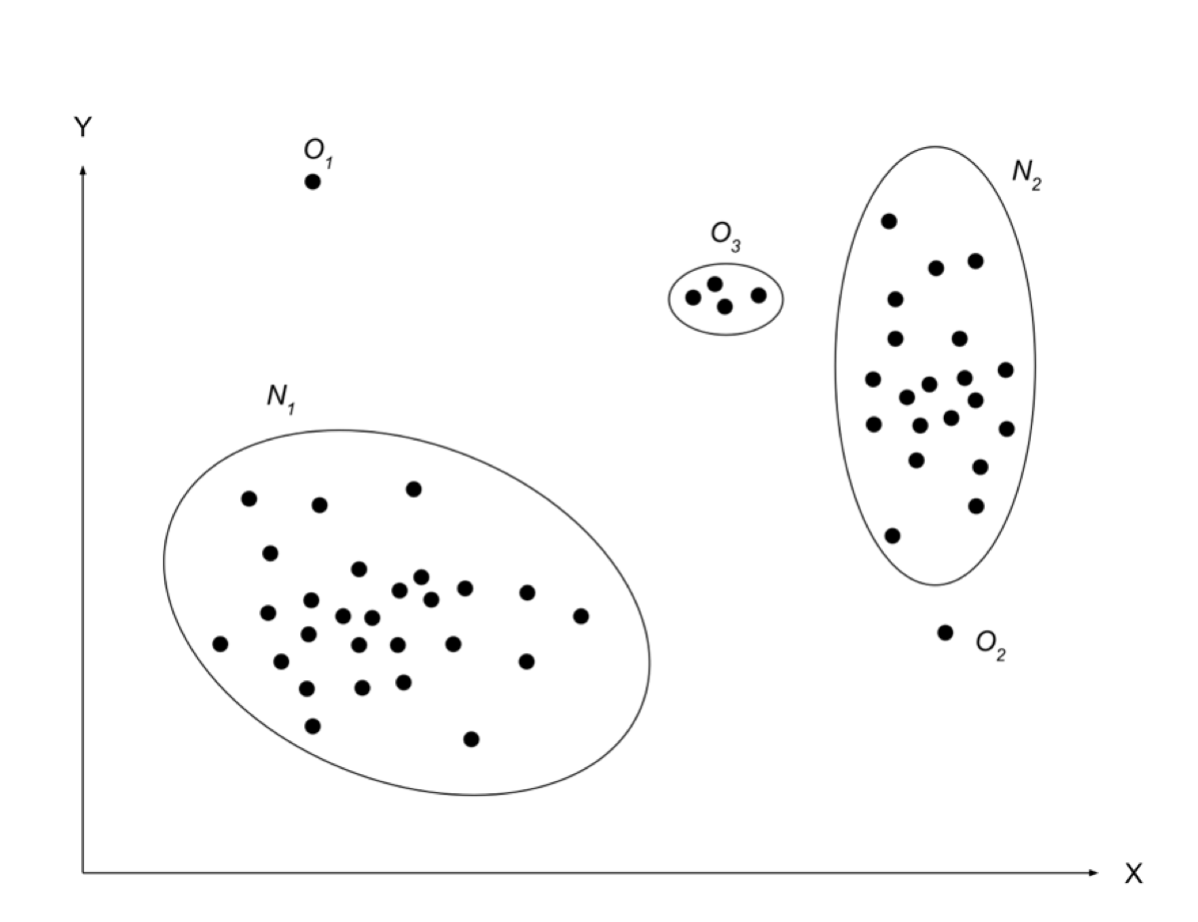
\includegraphics[scale=0.3]{images/anomalies.png}
% \caption{An illustration of anomalies in two-dimensional data set.}
% \label{fig:anomalies}
% \end{figure}

As illustrated in Figure ~\ref{fig:anomalies}, $N_{1}$ and $N_{2}$ are regions consisting of majority of observations and hence considered as normal data instance regions, whereas the region $O_{3}$, and data points  $O_{1}$ and $O_{2}$  are few data points which are located further away from the bulk of data points and hence are considered anomalies. Anomalies may arise due to several reasons, such as malicious actions, system failures, intentional fraud, etc. These anomalies reveal interesting insights about the data and are often convey valuable information about data. Therefore, anomaly detection considered an essential step in various decision-making systems.
% Novelty Detection Definition
% \begin{figure}[h]
% 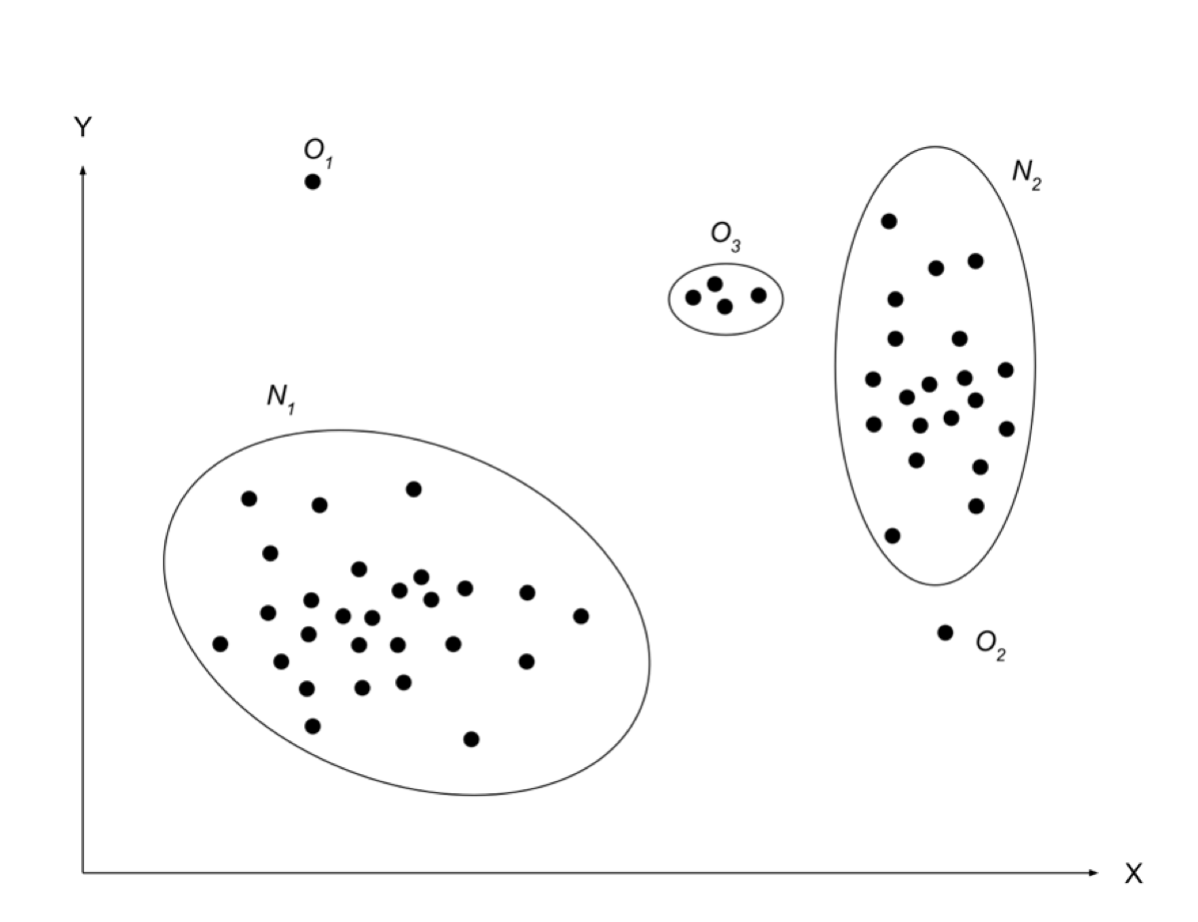
\includegraphics[scale=0.3]{images/anomalies.png}
% \caption{An illustration of anomalies in two-dimensional data set.}
% \label{fig:novelties}
% \end{figure}

% Begin of figure
\begin{figure}
  \centering
  \begin{minipage}{.48\linewidth}
    \centering
    % \subcaptionbox{}
      {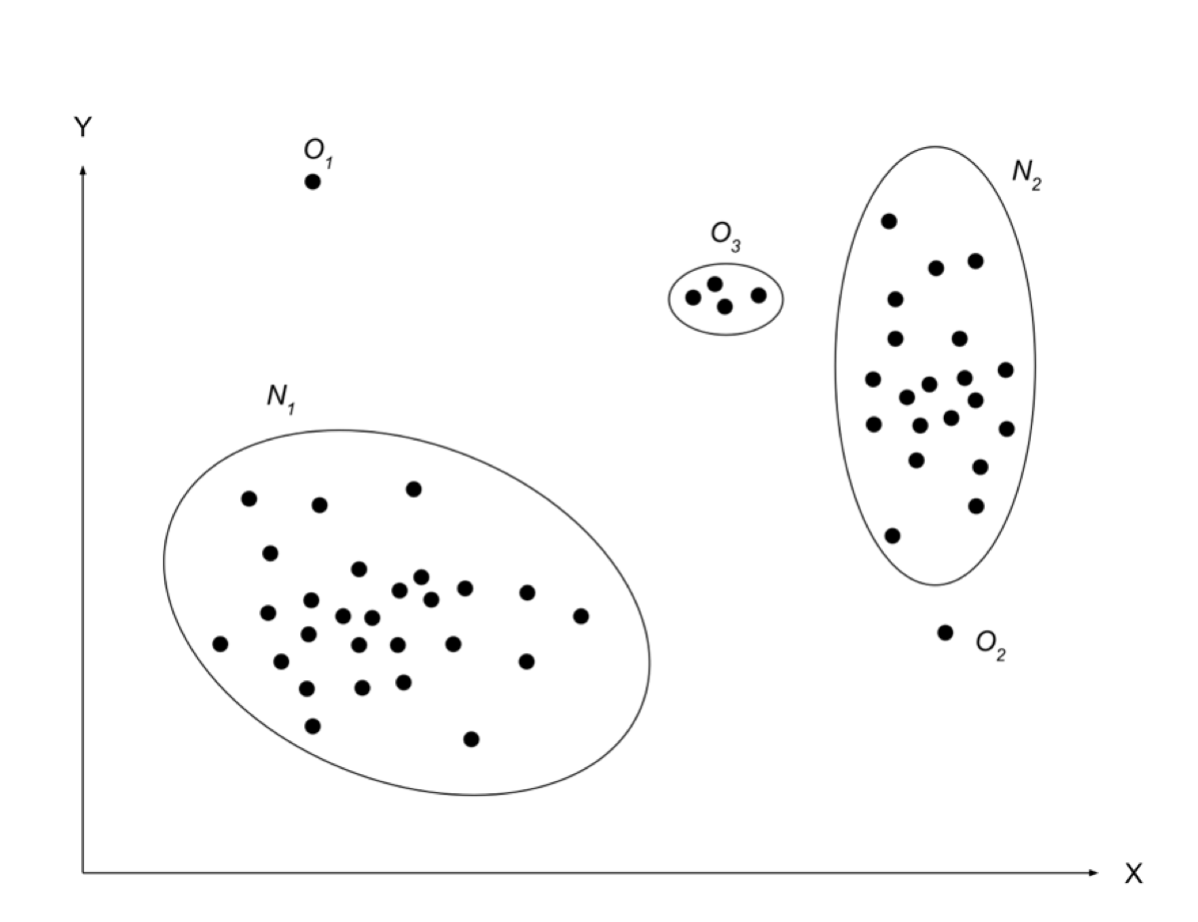
\includegraphics[scale=0.35]{images/anomalies.png}}
    \caption{Illustration of anomalies in two-dimensional data set.}
    \label{fig:anomalies}
  \end{minipage}\quad
  \begin{minipage}{.48\linewidth}
    \centering
    % \subcaptionbox{t}
      {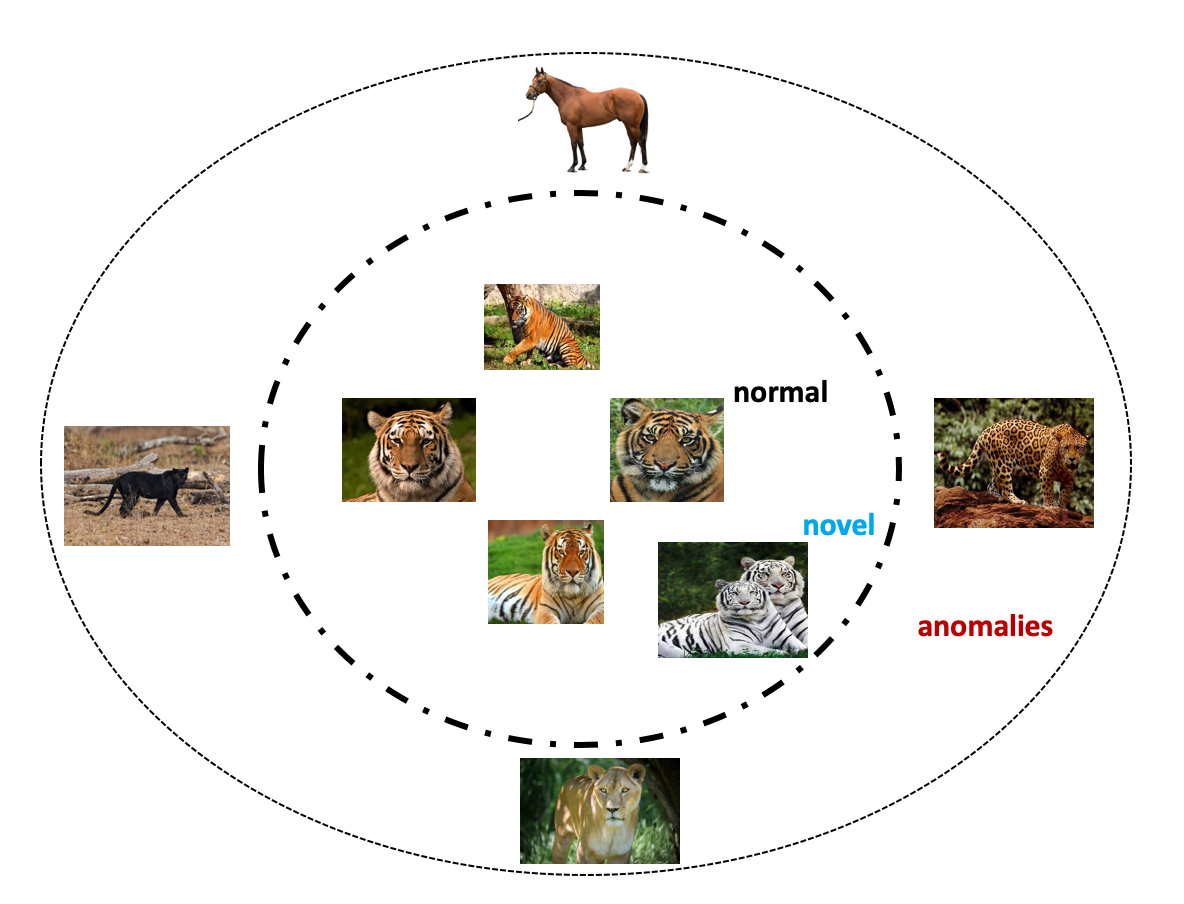
\includegraphics[scale=0.35]{images/novel.png}}
    \caption{Illustration of novelty in image data set.}
    \label{fig:novelties}
  \end{minipage}
  \bigskip

\end{figure}
% end of figure


% novelties
\subsection{What are novelties ?}
Novelty detection is the identification of novel (new) or unobserved patterns in the data.~\cite{miljkovic2010review}. The novelties detected are not considered as anomalous data points; instead they are incorporated into the normal data model. A novelty score may be assigned for these previously unseen data points, using a decision threshold score. ~\cite{pimentel2014review}.  The points which significanlty deviate from this decision threshold may be deemed as anomalies or outliers. For instance in Figure ~\ref{fig:novelties}  the images of \textit{(white tigers)} among normal tigers may be considered as novelty, while image of \textit{(horse, panther,lion and cheetah)} are considered as anomalies.
The techniques used for anomaly detection are often used for novelty detection and vice versa.



% Challenges : Motivation and challenges Why deep learning-based anomaly detection.
\subsection{Motivation and Challenges: Deep anomaly detection (DAD) techniques}
\begin{itemize}
\item Performance of traditional algorithms in detecting outliers is sub-optimal on complex image (e.g. medical images) and sequence data sets.
\item  Need for Large-scale anomaly detection : As the volume of data increases let's say to gigabytes then, it becomes nearly impossible for the traditional methods to scale to such large scale data to find outliers.
\item  Deep anomaly detection (DAD) techniques learn hierarchical discriminative features from data. This automatic feature learning capability eliminates the need of developing manual features by domain experts, therefore advocates to solve the problem end-to-end taking raw input data in domains such as text and speech recognition.
\item The boundary between normal and anomalous (erroneous) behavior is often not precisely defined  in several data domains and is constantly evolving. This lack of well defined representative normal boundary poses challenges for both conventional and deep learning-based algorithms.
\end{itemize}
% end itemize

% Begin Table
\begin{table} [ht!]
\centering
\captionsetup{justification=centering}
\caption{Comparison of our Survey to Other Related Survey Articles. 1 \textemdash Our Survey,\\
2 \textemdash Kwon and Donghwoon [2017],           5 \textemdash John and Derek [2017] \\
3 \textemdash Kiran  and Thomas [2018],            6 \textemdash Mohammadi and Al-Fuqaha [2017]\\
4 \textemdash Adewumi and Andronicus [2017]        7 \textemdash Geert and  Kooi et.al [ 2017].
}
\begin{tabular}{ |c|c|c|c|c|c|c|c|c|c| }
\hline
 & & 1&2&3&4&5&6&7 \\
\hline
\multirow{4}{6em}{Methods  }
&Supervised &\checkmark  & & & & & & \\
&Unsupervised &\checkmark & & & & & &  \\
&Hybrid Models & \checkmark& & & & & &  \\
&one-Class Neural Networks &\checkmark & & & & & &  \\
\hline
\multirow{8}{8em}{Applications  }
&Fraud Detection&\checkmark  & & &\checkmark & & & \\
&Cyber-Intrusion Detection&\checkmark  &\checkmark & & & & & \\
&Medical Anomaly Detection&\checkmark  & & & & & &\checkmark \\
&Sensor Networks Anomaly Detection&\checkmark  & & & &\checkmark & & \\
&Internet Of Things (IoT)
 Big-data Anomaly Detection&\checkmark  & & & & & \checkmark& \\
&Log-Anomaly Detection&\checkmark  & & & & & & \\
&Video Surveillance&\checkmark & &\checkmark  & & & & \\
&Industrial Damage Detection&\checkmark & & & & & & \\
\hline
\end{tabular}
\end{table}
% End of Table

% Related Work
\subsection{Related Work}
Despite the substantial advances made by deep learning methods in many machine learning problems, there
is a relative scarcity of deep learning approaches for anomaly detection. Adewumi et.al~\cite{adewumi2017survey} provide a comprehensive survey of deep learning-based methods for fraud detection. A broad review of deep anomaly detection (DAD) techniques for cyber-intrusion detection is presented by Kwon et.al~\cite{kwon2017survey}. An extensive review of using DAD techniques in medical domain has been presented by Litjens et.al ~\cite{litjens2017survey}. An  overview of DAD techniques for Internet of Things (IoT) and  big-data anomaly detection is introduced by  Mohammadi et.al~\cite{mohammadi2017deep}. Sensor networks anomaly detection has been reviewed  by  Ball et.al~\cite{ball2017comprehensive}. The state-of-the-art deep learning based methods for video anomaly detection along with various categories has been presented in~\cite{kiran2018overview}. Although there are a number of reviews in applying DAD technqiues, there is shortage of comparative analysis of deep learning architecture adopted for outlier detection. For instance a substantial amount of research on anomaly detection is conducted using deep autoencoders, but there is lack of comprehensive survey of various deep architecture's best suited for a given data-set and application domain. We hope that this survey bridges this gap and provides a comprehensive reference for researchers and engineers aspiring to leverage deep learning for anomaly detection. Table I shows the set of research methods and application domains covered by our survey.

% The classification taxonomy is also present in this paper $https://www.ncbi.nlm.nih.gov/pmc/articles/PMC4836738/$
% This paper~\cite{erfani2016high} presents a hybrid approach of combining deep learning models in combination with other traditional techniques to identify outliers and obtained promising results.

% Anomaly Detection Taxonomy
\begin{figure}[h]
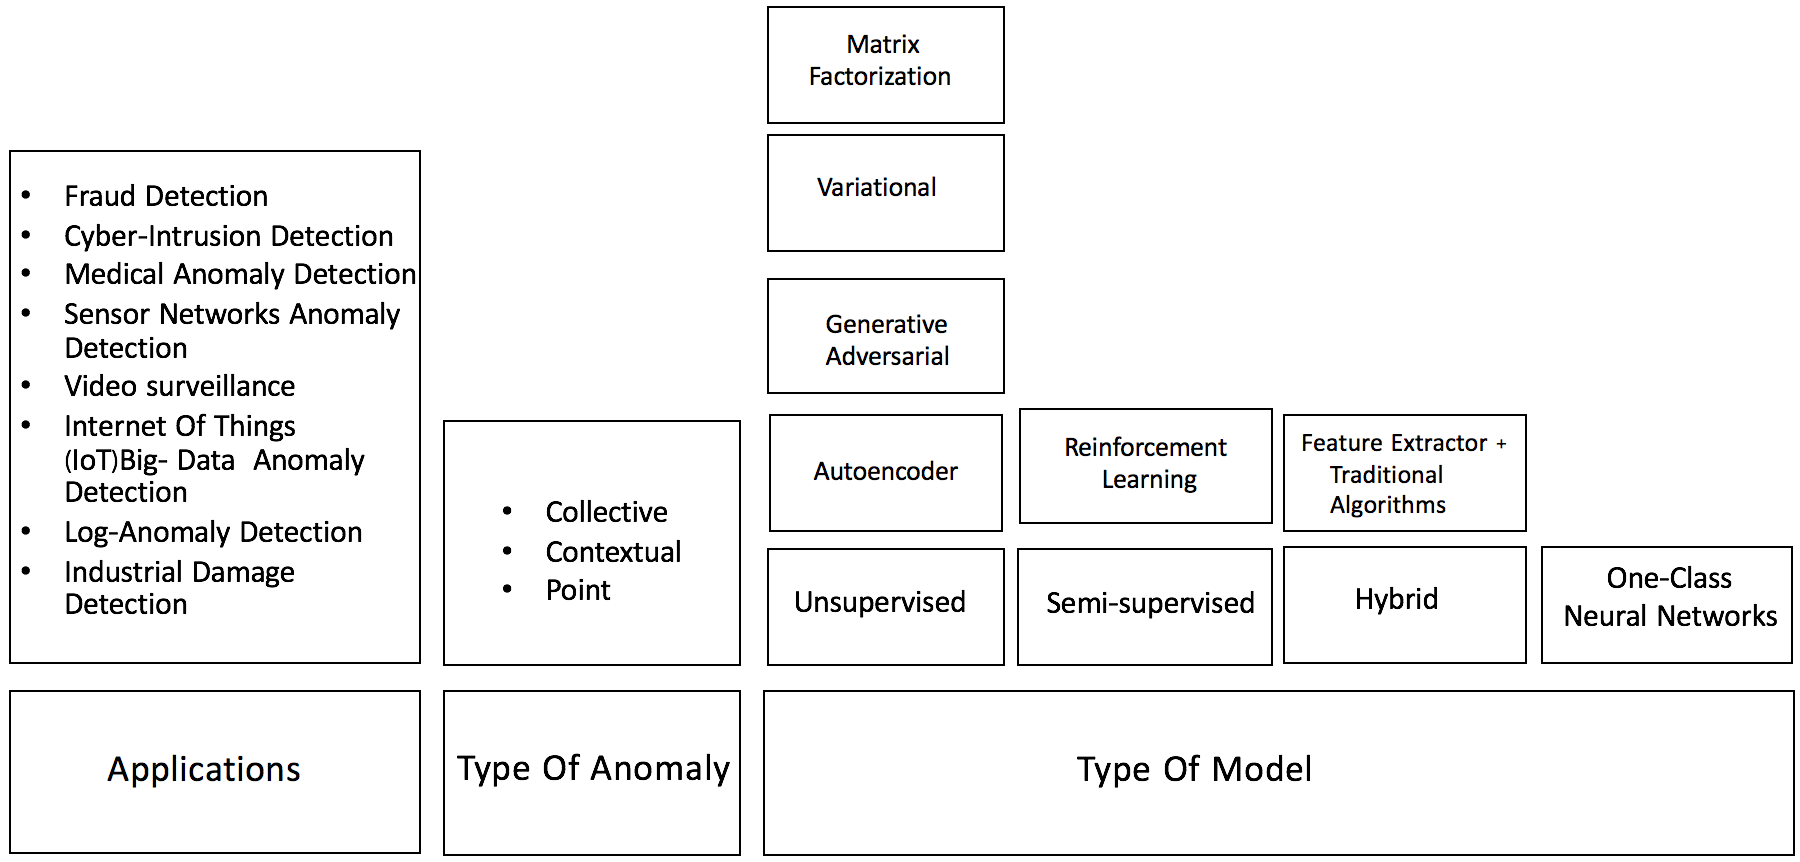
\includegraphics[scale=0.5]{images/AnomalyDetectionTaxonomy}
\caption{Key components associated with deep learning-based anomaly detection technique.}
\label{fig:surveyTaxonomy}
\end{figure}
% end of related work

%% Our Contributions
\subsection{ Our Contributions}
We follow survey approach of V.Chandola and A.Banerjee et.al~\cite{chandola2007outlier} for deep  anomaly detection (DAD). Our survey presents a detailed and structured overview of research and applications of DAD techniques. We summarize our main contributions as follows:
\begin{itemize}
\item Most of the existing surveys on DAD techniques either focus on a particular
application domain or specific research area of interest~\cite{kiran2018overview,mohammadi2017deep,litjens2017survey,kwon2017survey,adewumi2017survey,ball2017comprehensive}.
This review aims to provide a comprehensive outline of state-of-the art research in DAD techniques as well as several real world applications these techniques are discussed.
\item In recent years a number of new deep learning based anomaly detection techniques  with greatly reduced computational requirements have been developed. The purpose of this paper is to survey these techniques and classify them into organised schema for better understanding. We introduce two more sub-categories Hybrid models ~\cite{erfani2016high} and one-class neural networks techniques~\cite{chalapathy2018anomaly} as illustrated in Figure~\ref{fig:surveyTaxonomy} based on the choice of training objective. For each categories we discuss both the assumptions and techniques adopted for best performance. Furthermore within each category, we also present the challenges, advantages and disadvantages and provide an overview of computational complexity of DAD methods.
\end{itemize}

% Organization of the paper
\subsection{Organization}
This survey is organized by following structure described in Figure~\ref{fig:surveyTaxonomy}.
In Section~\ref{sec:aspectsOfAnomalyDetection}, we identify the various aspects that determine the formulation of the problem and highlight the richness and complexity associated with anomaly detection.
We introduce and define two types of models: contextual and collective or group anomalies. In Section~\ref{sec:applicationsOfDLAD}, we briefly describe the different application domains to which deep learning-based anomaly detection has been applied. In subsequent sections we provide a categorization of deep learning-based techniques based on the research area to which they belong.  Based on training objectives employed and availability of labels  deep learning-based anomaly detection techniques  can be categorized into supervised (Section~\ref{sec:supervisedDAD}), unsupervised (Section ~\ref{sec:unsupervisedDAD}), hybrid (Section~\ref{sec:hybridModels}), and one-class neural network  (Section~\ref{sec:oneclassNN}). For each category of techniques we also discuss their computational complexity for training and testing phases. In Section~\ref{sec:typeBasedAD} we discuss  point, contextual, and collective (group) deep learning-based anomaly detection techniques. We present some discussion of the limitations and relative performance of various existing techniques in Section~\ref{sec:relativeSOW}. Section~\ref{sec:conclusion} contains
concluding remarks.

